%\title{Presentation Template}
\documentclass[10pt]{beamer}

\usetheme[progressbar=frametitle]{metropolis}
\usepackage{appendixnumberbeamer}

\usepackage[compatibility=false]{caption}
\usepackage{subcaption}
\usepackage{csquotes}
\usepackage{booktabs}
\usepackage{hyperref}
\usepackage[scale=2]{ccicons}
\usepackage{tikz}
\usepackage{bm}

\usepackage{multimedia}
\usepackage{media9}

\graphicspath{{./img/}}

\usepackage{pgfplots}
\usepgfplotslibrary{dateplot}

\usepackage{xspace}
\newcommand{\themename}{\textbf{\textsc{metropolis}}\xspace}

\title{TITLE}
\subtitle{EVENT}
\date{DATE}
\author{Matthew Andres Moreno \newline \texttt{mmore500@msu.edu}}
\titlegraphic{\hfill
\includegraphics[height=2cm]{img/MSU-Wordmark-Black}}

\begin{document}

\maketitle

% \begin{frame}{Table of contents}
%   \setbeamertemplate{section in toc}[sections numbered]
%   \tableofcontents[hideallsubsections]
% \end{frame}

\section{Section}

\begin{frame}{Slide Title}
\begin{columns}
\begin{column}{0.6\textwidth}
\begin{itemize}
\item data management
\item foo
\end{itemize}
\end{column}
\begin{column}{0.4\textwidth}
\begin{center}
words
\end{center}
\end{column}
\end{columns}
\end{frame}

\begin{frame}{Youtube Video: Example}
\begin{figure}
  \includemedia[width=\linewidth,height=0.6\textwidth, flashvars={scaleMode=zoom}]{}{http://www.youtube.com/v/z9ptOeByLA4?t=1m08s&amp;rel=0&amp;showinfo=0}
  \captionsetup{singlelinecheck=off,justification=raggedright}
\caption{
Remember to use Adobe viewer!
\href{https://youtu.be/z9ptOeByLA4?t=1m08s}{(link)}
}
\end{figure}

\end{frame}


\appendix

\begin{frame}{For More Information}

\vspace{1ex}

{\HUGE\url{https://osf.io/ewvg8/}}

\vspace{3ex}

\begin{itemize}
\item live in-browser demo
\item source code
\item data
\item figures and graphics
\item how-to-replicate tutorial
\item publication
\item slides
\item blog article
\end{itemize}

\end{frame}

\begin{frame}{People}

\begin{columns}
\begin{column}{0.25\textwidth}
  \centering
  
\includegraphics[width=0.7\textwidth]{moreno}
\end{column}
\begin{column}{0.75\textwidth}
  \textbf{Matthew Andres Moreno}

  \href{https://twitter.com/MorenoMatthewA}{{\faTwitter} @MorenoMatthewA}

  \href{https://mmore500.github.io}{{\faGlobe} \texttt{https://mmore500.github.io}}

  \href{mailto: mmore500@msu.edu}{{\faEnvelope} \texttt{mmore500@msu.edu}}

\end{column}
\end{columns}

\vspace{1ex}

\begin{columns}
\begin{column}{0.25\textwidth}
  \centering
  \includegraphics[width=0.7\textwidth]{ofria}
\end{column}

\begin{column}{0.75\textwidth}
  \textbf{Charles Ofria}

  \href{https://twitter.com/CharlesOfria}{{\faTwitter} @CharlesOfria}

  \href{https://ofria.com}{{\faGlobe} \texttt{https://ofria.com}}

  \href{mailto: ofria@msu.edu}{{\faEnvelope} \texttt{ofria@msu.edu}}

\end{column}
\end{columns}
\vfill
\begin{columns}
\begin{column}{0.5\textwidth}
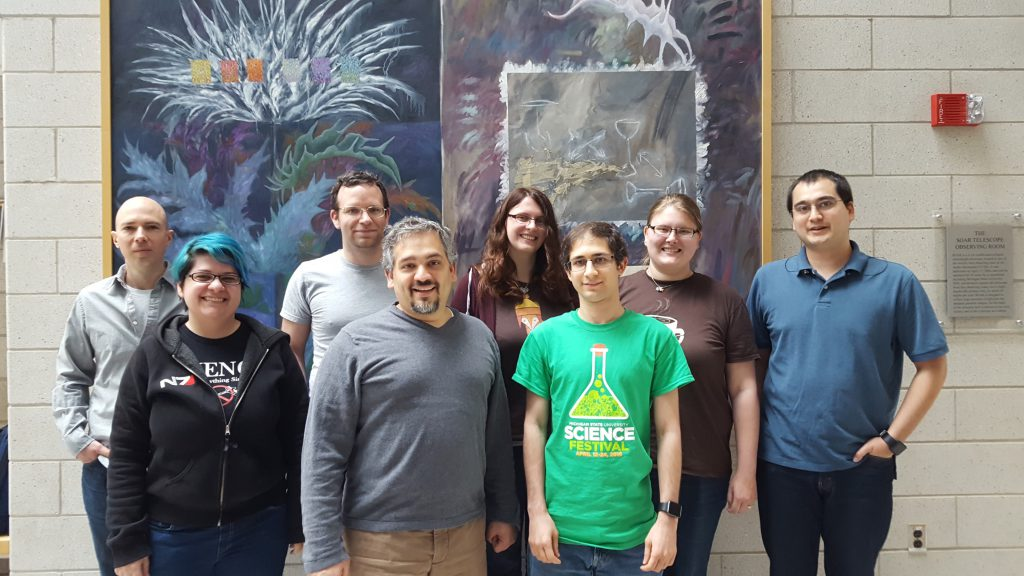
\includegraphics[width=\textwidth, trim={0 0 0 150}, clip]{group_photo}
\end{column}
\begin{column}{0.5\textwidth}

\includegraphics[width=\textwidth]{devolab-logo}
\end{column}
\end{columns}

\end{frame}

\begin{frame}{Acknowledgements}
\begin{itemize}
\item Empirical Library for scientific software development in C++
\item Open Science Framework via the Center for Open Science
\item computational resources via Michigan State University's Institute for Cyber-Enabled Research
\item This research was supported in part by NSF grants DEB-1655715 and DBI-0939454.\footnote[1]{Any opinions, findings, and conclusions or recommendations expressed in this material are those of the author(s) and do not necessarily reflect the views of the National Science Foundation.}
\end{itemize}

\vfill

\newcommand{\innerspacer}{0.07\textwidth}
\newcommand{\content}{0.24\textwidth}
\newcommand{\outerspacer}{0.07\textwidth}

\begin{center}
 \begin{columns}
	\begin{column}{\outerspacer}~\end{column}
	 \begin{column}{\content}
		
\includegraphics[width=\textwidth]{NSF-logo}
 	\end{column}
  \begin{column}{\innerspacer}~\end{column}
	 \begin{column}{\content}
		
\includegraphics[width=\textwidth]{BEACON-logo}
 	\end{column}
  \begin{column}{\innerspacer}~\end{column}
 	\begin{column}{\content}
   
\includegraphics[width=0.75\textwidth]{MSU-helmet}
 	\end{column}
 	\begin{column}{\outerspacer}~\end{column}
 \end{columns}
\end{center}

\end{frame}


\begin{frame}[standout]
  Questions?
\end{frame}

\begin{frame}[allowframebreaks]{References}

  \bibliography{bibl}
  \setbeamertemplate{bibliography item}{\insertbiblabel}
  \nocite{*} % Insert publications even if they are not cited in the poster
  \bibliographystyle{apalike}
\end{frame}


\begin{frame}{Multichannel Inheritance Outcomes}
  \begin{figure}
  \begin{subfigure}[b]{0.85\textwidth}
    \begin{columns}
    \begin{column}{0.05\textwidth}
      \caption{}~\\\vspace{0ex}~\\
      \label{fig:same_multichannel_offspring}
    \end{column}
    \begin{column}{0.95\textwidth}
      \colorbox{extralightgray}{
\includegraphics[width=\textwidth]{same_multichannel_offspring}}
  \end{column}
\end{columns}
  \end{subfigure}
  \begin{subfigure}[b]{0.85\textwidth}
      \begin{columns}
      \begin{column}{0.05\textwidth}
        \caption{}~\\\vspace{0ex}~\\
        \label{fig:new_lowchannel_offspring}
      \end{column}
      \begin{column}{0.95\textwidth}
        \colorbox{extralightgray}{
\includegraphics[width=\textwidth]{new_lowchannel_offspring}}
\end{column}
\end{columns}
  \end{subfigure}
  \begin{subfigure}[b]{0.85\textwidth}
      \begin{columns}
      \begin{column}{0.05\textwidth}
      \caption{}~\\\vspace{0ex}~\\
      \label{fig:new_highchannel_offspring}
      \end{column}
      \begin{column}{0.95\textwidth}
        \colorbox{extralightgray}{
\includegraphics[width=\textwidth]{new_highchannel_offspring}\vspace{-10ex}}
\end{column}
\end{columns}
  \end{subfigure}
  \caption{
  Allowed multichannel inheritance outcomes;
  (\subref{fig:same_multichannel_offspring}) identical level 1 and 2 channels,
  (\subref{fig:new_lowchannel_offspring}) new level 1 channel with identical level 2 channel, and
  (\subref{fig:new_highchannel_offspring}) new level 1 and 2 channels.
  }
\end{figure}

\end{frame}

\begin{frame}{Multichannel Inheritance: Hierarchy}%
  \textbf{hierarchy explicitly enforced:}
  \begin{itemize}
    \item no option to generate offspring w/ new Level 1 channel and same Level 2 channel
    \item thus, same Level 1 channel $\rightarrow$ same Level 2 channel
  \end{itemize}

  \pause

  \vspace{2ex}
  \textbf{analogy:}
  \begin{itemize}
    \item citizens of the same province $\rightarrow$ citizens of same country
  \end{itemize}

\end{frame}

\begin{frame}{Outcome: Evolution of Level-two Individuality}
\begin{figure}
\begin{columns}
\begin{column}{0.6\textwidth}
\includegraphics<1>[width=\textwidth]{results/ChannelMap_1011_update0.png}%
\includegraphics<2>[width=\textwidth]{results/ChannelMap_1011_update500000.png}%
\includegraphics<3>[width=\textwidth]{results/ChannelMap_1011_update1000000.png}%
\includegraphics<4>[width=\textwidth]{results/ChannelMap_1011_update2000000.png}%
\includegraphics<5>[width=\textwidth]{results/ChannelMap_1011_update4000000.png}%
\includegraphics<6>[width=\textwidth]{results/ChannelMap_1011_update5000000.png}%
\includegraphics<7>[width=\textwidth]{results/ChannelMap_1011_update7000000.png}%
\end{column}
\begin{column}{0.4\textwidth}
\only<1>{Update: 0}%
\only<2>{Update: 500,000}%
\only<3>{Update: 1,000,000}%
\only<4>{Update: 2,000,000}%
\only<5>{Update: 4,000,000}%
\only<6>{Update: 5,000,000}%
\only<7>{Update: 7,000,000}%

\vspace{8ex}

\caption{Channel-map visualization of a simulation where second-level individuality evolved.}
\end{column}
\end{columns}
\end{figure}
\end{frame}

\begin{frame}{Future Work: Biologically-Motivated}

investigate roles of following w.r.t. major evolutionary transitions:
\pause
\begin{itemize}[<+->]
\item  pre-existing phenotypic plasticity \cite{clune2007investigating, lalejini2016evolutionary}
\item pre-existing environmental interactions
\item pre-existing reproductive division of labor
\end{itemize}

\end{frame}


\end{document}
